% Latex version of the original catalog proposal document by santosiv@in.ibm.com,
% (C) 2015 IBM Corporation
% Confidential - Internal Use only

\documentclass[14]{article}
\usepackage[a4paper]{geometry}
\usepackage{fancyhdr}
\usepackage{graphicx}
\usepackage{placeins}
\usepackage[T1]{fontenc}

\makeatletter
\AtBeginDocument{%
  \expandafter\renewcommand\expandafter\subsection\expandafter
    {\expandafter\@fb@secFB\subsection}%
  \newcommand\@fb@secFB{\FloatBarrier
    \gdef\@fb@afterHHook{\@fb@topbarrier \gdef\@fb@afterHHook{}}}%
  \g@addto@macro\@afterheading{\@fb@afterHHook}%
  \gdef\@fb@afterHHook{}%
}
\makeatother

% with this we ensure that the chapter and section
% headings are in lowercase.
\renewcommand{\sectionmark}[1]{\markright{#1}}

\usepackage[colorlinks]{hyperref}
\usepackage[figure,table]{hypcap} % Correct a problem with hyperref

\hypersetup {
  colorlinks = true,
  urlcolor = black,
  pdfauthor = {Santosh Sivaraj <santosiv@in.ibm.com},
  pdfkeywords = {24x7, catalog, format},
  pdftitle = {24x7 Event and Group Catalog Formats Proposal},
  pdfsubject = {24x7 catalog},
  pdfpagemode = UseNone
}

\newgeometry{left=2cm,right=2cm,bottom=2cm}

\setlength{\parskip}{\baselineskip}%
\setlength{\parindent}{0pt}%

\begin{document}

\begin{center}

{ \huge \bfseries 24x7 Event and Group Catalog Formats Proposal \\[0.4cm] }

\end{center}
\noindent
\emph{Authors:}\\
Jim Benson (\texttt{jeben@us.ibm.com}) \\
Phil Vitale (\texttt{vit@us.ibm.com}) \\

\begin{center}
\emph{Approved on} 2013-05-14 (by common consent, version: v0.15) \\
\emph{Current Version:} v0.16 \\
\emph{Last Update:} \today
\end{center}

\pagebreak
\tableofcontents
\pagebreak

\section{Introduction}
The 24x7 Event and Group catalog is the performance counter consumer's
translator from “Event Name” to “Counter Data” through the PowerVM
H\_Get24x7Data hcall. Data available in the event entry or group entry in the
catalog is passed through the hcall so that the PowerVM can return the correct
data from the 24x7 “In Memory Accumulators”.

Clients looking for a specific counter's data, search the events array for a
matching event name. When found, the event entry will contain an IMA Group
Record Offset and an IMA Group Record Length. These two values, along with some
configuration specifics are passed to the PowerVM through the H\_Get24x7Data
hcall to retrieve the Event Group Record. The event entry also contains an
offset into the Event Group Record where the desired counter can be found.

Often clients want a group of event counters so that together more complex
metrics can be computed. Clients will search the groups array for a matching
group name. When found the group entry will, like the event entry, contain an
IMA Group Record Offset and an IBM Group Record Length. These two values, along
with some configuration specifics are passed to the PowerVM through the
H\_Get24x7Data hcall to retrieve the Event Group Record. The group entry also
contains a list of event entry indexes so that the offsets (found through the
event entry) can be use to retrieve desired counters from the Event Group
Record.

The figure below illustrates these relationships.

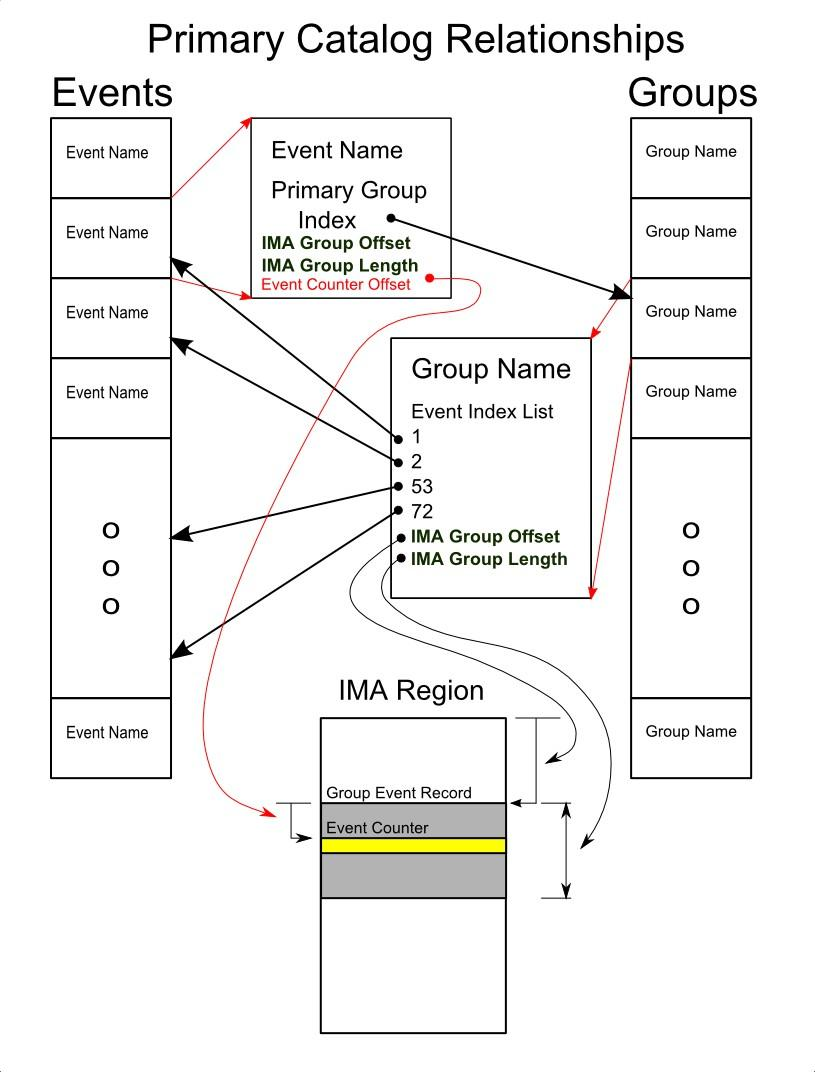
\includegraphics[scale=0.6]{primary_catalog_relationships.jpeg}

\pagebreak

\section{Catalog Page 0}
\begin{tabular}[l]{|p{5cm}|c|p{7cm}|}
\hline
\textbf{Field} & \textbf{Byte Offset} & \textbf{Attributes} \\
\hline
Descriptor & 0x00 & uint32 "24x7" in ASCII \\
\hline
Length & 0x04 & uint32 (in 4096 byte pages) \\
\hline
Version Number & 0x08 & uint64 \\
\hline
Build Date-stamp & 0x10 & char[16] Zero-terminated ASCII string → YYYYMMDDHHMMSS \\
\hline
Reserved & 0x20 & char[32] \\
\hline
Offset to Schema Data & 0x40 & uint16 (in 4096 byte pages) \\
\hline
Length of Schema Data & 0x42 & uint16 (in 4096 byte pages) \\
\hline
Schema Entry Count & 0x44 & uint16 \\
\hline
Reserved & 0x46 & char[2] \\
\hline
Offset to Event Data & 0x48 & uint16 (in 4096 byte pages) \\
\hline
Length of Event Data & 0x4A & uint16 (in 4096 byte pages) \\
\hline
Event Entry Count & 0x4C & uint16 \\
\hline
Reserved & 0x4E & char[2] \\
\hline
Offset to Group Data & 0x50 & uint16 (in 4096 byte pages) \\
\hline
Length of Group Data & 0x52 & uint16 (in 4096 byte pages) \\
\hline
Group Entry Count & 0x54 & uint16 \\
\hline
Reserved & 0x56 & char[2] \\
\hline
Offset to Formula Data & 0x58 & uint16 (in 4096 byte pages) \\
\hline
Length of Formula Data & 0x5A & uint16 (in 4096 byte pages) \\
\hline
Formula Entry Count & 0x5C & uint16 \\
\hline
Reserved & 0x5E & char[2] \\
\hline
Offset to core events & 0x60 & u32 Offset relative to the main event group (0x48)\\
\hline
Offset to thread events & 0x64 & u32 Offset relative to the main event group (0x48)\\
\hline
Offset to chip events & 0x68 & u32 Offset relative to the main event group (0x48)\\
\hline
Offset to core group & 0x6C & u32 Offset relative to the main group data (0x50) \\
\hline
Offset to thread group & 0x70 & u32 Offset relative to the main group data (0x50) \\
\hline
Offset to chip group & 0x74 & u32 Offset relative to the main group data (0x50) \\
\hline
Reserved & 0x78 & char[8] \\
\hline
\end{tabular}

\textit{Design Note:} The “Length” field and “Version Number” size and offset is fixed
since the hypervisor will fill in the Length when the catalog is read from the
fsp flash lid table and will compare the Version Number for consistency on each
hypervisor call. The offset to the events and groups are relative to the main
event group page and the group data page. In cases where there are no group for
particular sub-group (like thread or chip), the offset at such field will be
filled with '0xffffffff' to mark it as invalid.

\subsection{Example Catalog Page0 Raw Data}
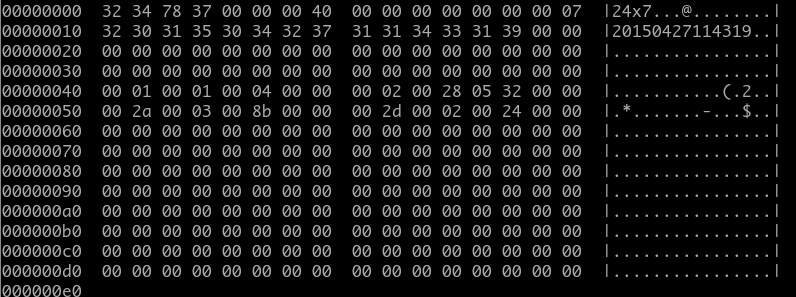
\includegraphics[scale=0.6]{page0_raw.png}

\pagebreak

\section{Event Data}
\begin{tabular}[l]{|p{5cm}|c|p{7cm}|}
  \hline
  \textbf{Field} & \textbf{Byte Offset} & \textbf{Attributes} \\
  \hline
  Event Structure Length (in bytes) & 0x00 & uint16 - Structure will be padded 
                                             with zeros to create a structure
                                             with a length which is an even
                                             multiple of 16 \\
  \hline
  Reserved & 0x02 & char[2] \\
  \hline
  IMA Group Record Domain & 0x04 & uint8 - ( Chip = 1 / Core = 2 / Thread PMU = 3
                                   ) \\
  \hline
  Reserved & 0x05 & char[1] \\
  \hline
  Byte offset to Start of Event Group Record & 0x06 & uint16 - (must be 8-byte
                                                      aligned) \\
  \hline
  Byte length of entire Event Group Record & 0x08 & uint16 \\
  \hline
  Byte offset in Event Group Record to Event Counter & 0x0A & uint16 \\
  \hline
  \parbox[t]{5cm} {
  Flag:
  \begin{itemize}
    \renewcommand\labelitemi{--}
    \setlength\itemsep{-0.4em}
    \item Verified-State
    \item Unverified-State
    \item Caveat-State
    \item Broken-State
    \item Mask Bits ("gated-by" MSR states, info only)
    \end{itemize}
  } & 0x0C & uint32 - (binary composition) \\
  \hline
  Reserved & 0x0C & uint32 - (binary composition) \\
  \hline
  Primary Group Index & 0x10 & uint16 - Index into the Group Data array where
                               either the first or best group which contains this
                               event can be found \\
  \hline
  Group Count & 0x12 & uint16 - Number of groups which this event is a part of \\
  \hline
  Event Name Field Length & 0x14 & uint16 – (n1) This length includes the length
                                   of the Event Name Field Length field \\
  \hline
  Event Name & 0x14 + 2 & char[] - Variable (zero-terminated ASCII padded to
                          half-word length) \\
  \hline
  Event Description Field Length & 0x14 + n1 & uint16 – (n2) If there there is no
                                               Event Description or the Event
                                               Description is the same as the
                                               Event Name, then this length
                                               will be 2 (length of length
                                               field). \\
  \hline
  Event Description & 0x14 + n1 + 2 & char[] - Variable (zero-terminated ASCII
                                      padded to half-word length) \\
  \hline
  Event Detailed Description Field Length & 0x14 + n1 + n2 & uint16 - (n3) If
                                                             there there is no
                                                             Event Detailed
                                                             Description or the
                                                             Event Detailed
                                                             Description is the
                                                             same as the Event
                                                             Description, then
                                                             this length will be
                                                             2 (length of length
                                                             field). \\
  \hline
  Event Detailed Description & 0x14 + n1 + n2 + 2 & char[] - Variable (zero-
                                                    terminated ASCII padded to
                                                    half-word length) \\
  \hline
\end{tabular}

\subsection{Event Data Entry Notes}
\begin{itemize}
\item The “Event Name Field Length”, “Event Description Field Length” and “Event
  Detailed Description Field Length” fields INCLUDE the length of the length
  field. To point to the start of the next field's length add the current
  field's length. Thus a field length value of 2 indicates the text string is
  empty.
\item For events that are being accumulated in chip groups, each event will have
  an accumulated counter value and a “Last Sample Increment” value. The short
  name for the event which returns the “Last Sample Increment” will merely be
  the accumulated counter's Event Name with the “\_SAMPLE” suffix added. The
  “Last Sample Increment” event data will not have an event description or a
  detailed event description.
\item There are two, special core level events: HPM\_NON\_IDLE\_INST and
  HPMC\_NON\_IDLE\_PCYC which are available in all core groups in the
  GRS\_COUNTER\_3 and GRS\_COUNTER\_4 schema ENUM positions.
\item For some events that are being accumulated in core groups, those events
  will have counter versions available which are filtered by “context
  state”. For those events with a “filtered by user” state counter available,
  the event name will have the suffix \_USER appended. For those events with a
  “filtered by kernel” state counter available, the event name will have the
  suffix \_KERNEL appended. The “filtered” event data will not have an event
  description or a detailed event description.
\end{itemize}

\subsection{Example Event Entry Raw Data}
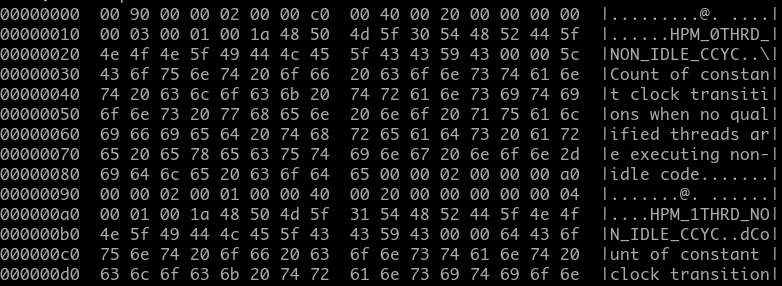
\includegraphics[scale=0.6]{events_raw.png}

\pagebreak

\section{Group Data}
\begin{tabular}[l]{|p{5cm}|c|p{7cm}|}
  \hline
  \textbf{Field} & \textbf{Byte Offset} & \textbf{Attributes} \\
  \hline
  Group Structure Length (in bytes) & 0x00 & uint16 - Structure will be padded
                                             with zeros to create a structure
                                             with a length which is an even
                                             multiple of 16 \\
  \hline
  Reserved & 0x02 & char[2] \\
  \hline
  \parbox[t]{5cm} {
  Flag:
  \begin{itemize}
    \renewcommand\labelitemi{--}
    \setlength\itemsep{-0.4em}
  \item Verified-State
  \item Unverified-State
  \item Caveat-State
  \item Broken-State
  \end{itemize}
  } & 0x04 & uint32 - (binary composition) NOTE: The “State” flags are merely
               a composite of the events in this group. The “worst” event will
               dictate the state of this group. \\
  \hline
  IMA Group Record Domain & 0x08 & uint8 - ( Chip = 1 / Core = 2 ) \\
  \hline
  Reserved & 0x09 & char[1] \\
  \hline
  Byte offset to Start of Event Group Record & 0x0A & uint16 - (must be 8-byte
                                                      aligned) \\
  \hline
  Byte length of entire Event Group Record & 0x0C & uint16 \\
  \hline
  Group Schema Index & 0x0E & uint8 – Use this index to find the schema which
                              describes the layout of this group's structure. \\
  \hline
  Event Count & 0x0F & uint8 - ( between 1 and 16 ) \\
  \hline
  Event Indexes & 0x10 & uint16[16] - (Index into Event Data array) \\
  \hline
  Group Name Field Length & 0x30 & uint16 – (n1) This length includes the length
                                   of the Group Name Field Length field \\
  \hline
  Group Name & 0x30 + 2 & char[] - Variable (zero-terminated ASCII padded to
                          half-word length) \\
  \hline
  Group Description Field Length & 0x30 + n1 & uint16 – (n2) If there there is no
                                               Group Description or the Group
                                               Description is the same as the
                                               Group Name, then this length
                                               will be 2 (length of length
                                               field). \\
  \hline
  Group Description & 0x30 + n1 + 2 & char[] - Variable (zero-terminated ASCII
                                      padded to half-word length) \\
  \hline
\end{tabular}

\subsection{Group Data Entry Notes}
\begin{itemize}
\item The “Group Name Field Length” and “Group Description Field Length” fields
  INCLUDE the length of the length field. To point to the start of the next
  field's length add the current field's length. Thus a field length value of 2
  indicates the text string is empty.
\item The Event Indexes array may contain “FREE” or “Unassigned” slots for
  future events. These slots will be recognized by the value -1 (0xFFFF) as the
  Event Index.
\end{itemize}

\subsection{Example Group Entry Raw Data}
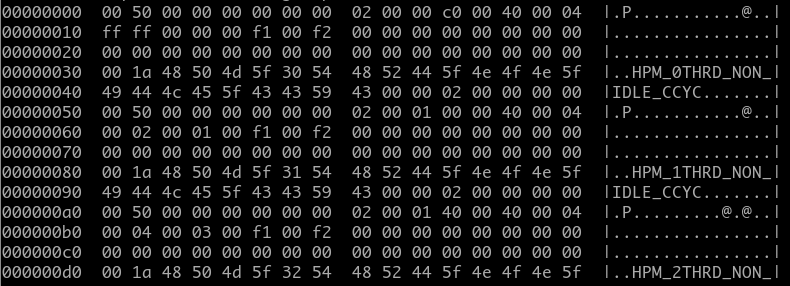
\includegraphics[scale=0.6]{groups_raw.png}

\textit{NOTE:} At the moment, the core (HPMC) groups have not been named... these
group names are merely the name of the first event of the group.

\pagebreak

\section{Schema Data}
These schemas are the same ones proposed in the 24x7 Requirements Document.

\subsection{Core and Chip Event Counter Group Record}
The Event Counter Group Record is a structure in memory containing the event
counters and administrative data accumulated by the hardware. The layout of this
structure is fixed in hardware, but is not guaranteed to be common across all
hardware processor versions or families.

Refer to the PORE/SLW workbook for the exact definition of this structure, but
examples of these structures can be found below.

\begin{table}
  \parbox{.45\linewidth}{
    \centering
    \begin{tabular}[l]{|c|c|}
      \hline
      \multicolumn{2}{|c|}{Timebase} \\ \hline
      \multicolumn{2}{|c|}{Number of Updates} \\ \hline
      \multicolumn{2}{|c|}{Group Measurement Period} \\ \hline
      \multicolumn{2}{|c|}{HPMC1} \\ \hline
      \multicolumn{2}{|c|}{HPMC2} \\ \hline
      \multicolumn{2}{|c|}{HPMC3 (sum NON\_IDLE\_INST)} \\ \hline
      \multicolumn{2}{|c|}{HPMC4 (sum NON\_IDLE\_PCYC)} \\ \hline
      Status [0:15] & Timebase [16:63] \\
      \hline
    \end{tabular}
    \caption{HPMC-IMA Core Domain Record (One "HPMC Group")}
  }
  \hfill
  \parbox{.45\linewidth}{
    \centering
    \begin{tabular}[l]{|c|}
      \hline
      Time-Of-Day (SCOM) \\ \hline
      Update Count \\ \hline
      Accumulated Measurement Period \\ \hline
      Accumulated pmulet-0 \\ \hline
      \dots \\ \hline
      Accumulated pmulet-N \\ \hline
      Last Update Period \\ \hline
      Last pmulet-0 Increment \\ \hline
      \dots \\ \hline
      Last pmulet-N Increment \\ \hline
      Time-Of-Day \\ \hline
    \end{tabular}
    \caption{PRE-SLW-IMA Chip Domain Record (One "pmulet Group")}
  }
\end{table}

The layout of an event counter group record is communicated dynamically through
a structure returned in the Get Event Counter Group Schema interface called the
Event Counter Group Schema. The structure used to accumulate counters in core
event group records differs from the structure used to accumulate counters in
chip event group records. Among the chip event group records, structure sizes
may differ. The Group Schema Index in the catalog group data entry indicates
which schema to use.

\subsection{Core and Chip Event Counter Group Record Schema
(GRS)}
The Event Counter Group Record Schema is a structure returned by the Get Event
Counter Group Record Schema hypervisor interface. This structure indirectly
defines the Event Counter Group Record using architected ENUMs, offsets and
lengths.

\begin{table}[hd]
  \begin{tabular}[l]{|p{5cm}|c|p{7cm}|}
    \hline
    \textbf{Field} & \textbf{Byte Offset} & \textbf{Attributes} \\
    \hline
    Schema Structure Length in bytes & 0x00 & uint16 - Structure will be padded
                                              with zeros to create a structure
                                              with a length which is an even
                                              multiple of 16 \\ \hline
    Reserved & 0x02 & char[2] \\ \hline
    Schema Descriptor & 0x04 & uint16 \\ \hline
    Schema Version Id & 0x06 & uint16 \\ \hline
    Reserved & 0x08 & char[6] \\ \hline
    Field Entry Count & 0x0E & uint16 \\ \hline
    Field Entries & 0x10 & char[0] - (first Group Record Schema Field begins here)
    \\ \hline
  \end{tabular}
  \caption{Group Record Schema}

  \begin{tabular}[l]{|p{5cm}|c|p{7cm}|}
    \hline
    \textbf{Field} & \textbf{Byte Offset} & \textbf{Attributes} \\
    \hline
    Field Enum & 0x00 & uint16 \\ \hline
    Offset into Event Counter Group Record & 0x02 & uint16 \\ \hline
    Field Length in Bytes & 0x04 & uint16 \\ \hline
    Flags/Reserved & 0x06 & uint16 – (binary composition) \\ \hline
  \end{tabular}
  \caption{Group Record Schema Field}
\end{table}

The “Field Enum” values will be consistent as the hardware design changes. If
any part of the structure changes, the Schema Version Id will change.

OS implementations are free to define fixed structures that will only apply to
known schema versions.

\subsection{Group Record Schema Field Content ENUMs}
\begin{tabular}[l]{lr}
  GRS\_COUNTER\_1 & 1 \\
  GRS\_COUNTER\_2 & 2 \\
  GRS\_COUNTER\_3 & 3 \\
  GRS\_COUNTER\_4 & 4 \\
  GRS\_COUNTER\_5 & 5 \\
  GRS\_COUNTER\_6 & 6 \\
  \multicolumn{2}{c}{\dots} \\
  GRS\_COUNTER\_31 & 31 \\
  GRS\_TIMEBASE\_UPDATE & 48 \\
  GRS\_TIMEBASE\_FENCE & 49 \\
  GRS\_UPDATE\_COUNT & 50 \\
  GRS\_MEASUREMENT\_PERIOD & 51 \\
  GRS\_ACCUMULATED\_MEASUREMENT\_PERIOD & 52 \\
  GRS\_LAST\_UPDATE\_PERIOD & 53 \\
  GRS\_STATUS\_FLAGS & 54 \\
\end{tabular}

\subsection{Group Record Schema ENUMs}
\begin{tabular}[l]{lr}
  GRS\_CORE\_SCHEMA\_INDEX & 0 \\
\end{tabular}

\subsection{Example Group Record Schema Entry Raw Data}
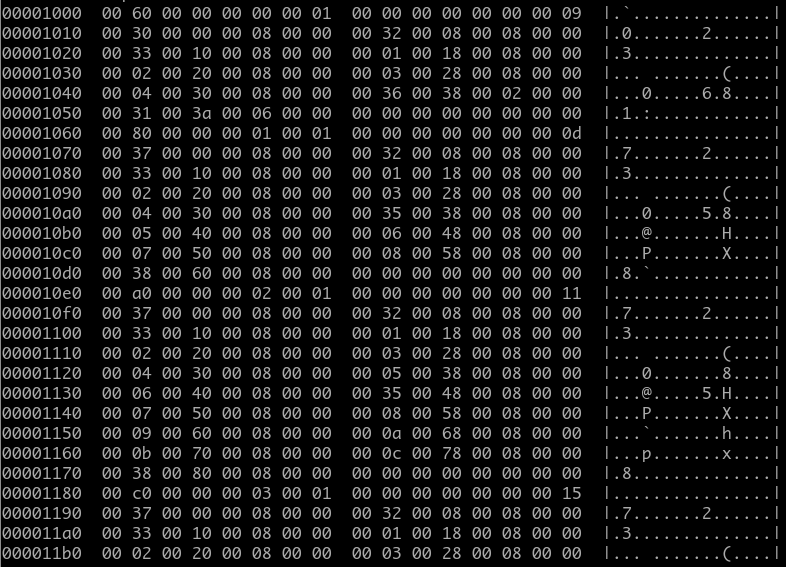
\includegraphics[scale=0.6]{group_schema_raw.png}

\pagebreak

\section{Formula Data}
\begin{tabular}[l]{|p{5cm}|c|p{7cm}|}
  \hline
  \textbf{Field} & \textbf{Byte Offset} & \textbf{Attributes} \\
  \hline
  
  Formula Structure Length (in bytes) & 0x00 & uint16 Structure will be padded with
                                               zeros to create a structure with
                                               a length which is an even
                                               multiple of 16 \\ \hline
  Reserved & 0x02 & char[2] \\ \hline
  \parbox[t]{5cm} {
  Flag:
  \begin{itemize}
    \renewcommand\labelitemi{--}
    \setlength\itemsep{-0.4em}
  \item Verified-State
  \item Unverified-State
  \item Caveat-State
  \item Broken-State
  \item Grouped
  \item Reserved
  \end{itemize}
  } & 0x04 & uint32 (binary composition) NOTE: The ``State'' flags are
             merely a composite of the events in this formula. The “worst”
             event will dictate the state of thisformula. \\ \hline
  Group & 0x08 & uint16 (if flag Grouped is TRUE) This is the group index where
                 all the formula's dependent events can be found. \\ \hline
  Reserved & 0x0A & char[6] \\ \hline
  Formula Name Field Length & 0x10 & uint16 (n1) - This length includes the
                                     length of the Formula Name Field Length
                                     field \\ \hline
  Formula Name & 0x10 & + 2 char[] Variable (zero-terminated ASCII padded to
                        half-word length) \\ \hline
  Formula Description Field Length & 0x10 & + n1 uint16 (n2) - This length
                                            includes the length of the Formula
                                            Description Field Length field \\
  \hline
  Formula Description & 0x10 + n1 + 2 & char[] Variable (zero-terminated ASCII
                                        padded to half-word length) \\ \hline
  Formula Field Length & 0x10 + n1 + n2 & uint16 (n3) - This length includes the
                                          length of the Formula Field Length
                                          field \\ \hline
  Formula & 0x10 + n1 + n2 + 2 & char[] Variable (zero-terminated ASCII padded to
                                 half-word length) NOTE: This formula field is
                                 intended to comply with a formula syntax that
                                 should make parsing and interpretation
                                 easier... see Formula Syntax below \\ \hline
\end{tabular}

\subsection{Formula Entry Notes}
\begin{itemize}
\item The ``Formula Name Field Length'', ``Formula Description Field Length'' and
  ``Formula Field Length'' fields INCLUDE the length of the length field. To point
  to the start of the next field's length add the current field's length. Thus a
  field length value of 2 indicates the text string is empty.
\end{itemize}

\subsection{Formula Syntax}
The Formula Field of a Formula Data Record will contain text that complies with
a simple syntax that should make parsing and interpretation easier.

The text will follow a general ``stack-based'', ``Reverse Polish Notation'' (or
``Post-fix Notation'' evaluation model generalized this way:

\begin{center}
  \texttt{
    operand [ operand | operator [ operand | operator ] [ \dots ] ]
  }
\end{center}

Where:
\begin{itemize}
\item Operand is either a text Event Name which can be found among the Event
  Data records, another Formula Name, a constant in standard floating point
  representation or a symbolic constant familiar to performance analysts such as
  'delta-timebase', 'delta-cycles', 'delta-instructions', and 'delta-seconds'.
\item Operator is any of the standard mathematical text characters: '+', '-',
  '*', or '/', or these lowercase, three-character mathematical abbreviations:
  'mod', 'rem', 'sqr', or 'x\^{}y', or these three-character stack manipulators:
  'swp', 'rot', and 'dup'.

\end{itemize}
Note that most operators require two operands, but some only require one.

Also be aware that most formulas can be extended to aggregate chips or cores if
the operands are first properly summed across all the domain resources of
interest.

To evaluate a formula, the interpreter implements a push-up operand stack where
new operands are added to the bottom of the stack (the x register) and operators
consume or manipulate the bottom-most operand and potentially (in the case of
two-operand operators) the operand immediately above the bottom (the y
register), placing the result back on the bottom of the stack. When the formula
interpretation is complete, the final result will be left at the bottom of the
stack.

\textit{Note:} Existing pmlist data represents formulas using standard “infix”
notation. For example:

\begin{verbatim}
# pmlist -DPMD_CPU_UTIL
Derived Metric: PMD_CPU_UTIL (unit:%) (CPU Utilization)
Formula : PM_RUN_CYC / PM_CYC * 100
Description :
Metric Groups : General
Groups : 0
\end{verbatim}

\subsubsection{Formula Operands}
\begin{center}
\begin{tabular}[l]{|l|p{7cm}|}
\hline
\textbf{Operand} & \textbf{Description} \\ \hline
Event Name & The value of this operand is a 24x7 counter accessed using data
             found in the Event Data table \\ \hline
Formula Name & The value of the operand is a computed metric derived using a
               formula found in the Formula Data table \\ \hline
Constant & A standard floating point constant \\ \hline
delta-timebase & The elapsed time in partition timebase ticks \\ \hline
delta-cycles & The elapsed clock cycles \\ \hline
delta-instructions & The elapsed instruction cycles \\ \hline
delta-seconds & The elapsed wall-time in seconds \\ \hline
\end{tabular}
\end{center}

\subsubsection{Formula Operators}
\begin{center}
\begin{tabular}[l]{|l|l|l|}
\hline
\textbf{Operator} & \textbf{Operands Consumed} & \textbf{Result} \\ \hline
+ & 2 (x, y) & x <= y + x \\ \hline
- & 2 (x, y) & x <= y - x \\ \hline
* & 2 (x, y) & x <= y * x \\ \hline
/ & 2 (x, y) & x <= y / x \\ \hline
mod & 2 (x, y) & x <= y \% x \\ \hline
rem & 2 (x, y) & x <= y // x \\ \hline
sqr & 1 (x) & x <= sqrt( x ) \\ \hline
x \^{} y & 2 (x, y) & x <= x \^{} y \\ \hline
swp & 2 (x, y) & x <= y, y <= x \\ \hline
rot & n (x..n) & x <= y, y <= z, ... n <= x (stack rotation) \\ \hline
dup & 1 (x) y & <=x, x <= x (duplicate bottom of stack) \\ \hline


\end{tabular}
\end{center}

\section{Related Documents}
\begin{center}
\begin{tabular}[l]{|p{7cm}|l|}
  \hline
  \href{https://mcdoc.boeblingen.de.ibm.com/out/out.Login.php?forward=/out/out.ViewDocument.php?documentid=2944}{P8
  Hypervisor 24x7 Interfaces} & Mike Vance \\
  \hline
\end{tabular}
\end{center}
Click on the document name to open the document in the web browser.

\pagebreak

\section{Change History}
\begin{center}
\begin{tabular}[l]{|l|l|p{10cm}|}
\hline
\textbf{Version} & \textbf{Date} & \textbf{Description} \\ \hline
  v0.10 & 2013-03-12 & Original draft \\ \hline
  v0.11 & 2013-03-20 & 
                       \parbox[t]{7cm} {
                       Corrections from John Attinella \\
  Addition of several flags similar to those used in PMC Event filtering \\
  Addition of the Group Index and Group Count fields to the Eventdata catalog
  record \\
  } \\ \hline
  v012 & 2013-03-28 & Added the concept of "derived metrics" through "named
                      formulas" using an additional "Formula Data" table. \\ \hline
  v0.13 & 2013-04-22 & Added build date-stamp to catalog. Clarified that there
                       may be several schemas to describe the various chip event
                       group records. Added a group record length to the event
                       data to save having to look up the length. \\ \hline
  v0.14 & 2013-04-24 & Added the same domain, group offset and length data
                       necessary to locate individual events to the group table
                       entry. Moved entry counts to Page 0 \\ \hline
  v0.15 & 2013-05-21 & Ooops! Mike Vance corrected me on the catalog version length.
                       Removed Questions section and marked as approved by common
                       consent. Typos. \\ \hline

  v0.16 & 2015-04-27 & santosiv@in.ibm.com - New fields in Page 0 structure and
                       a new domain for the thread groups \\ \hline
\end{tabular}
\end{center}
\end{document}
